\documentclass[a4paper]{article}
% Leave uncommented if the LaTeX file is uploaded to arXiv.org
\pdfoutput=1
\pdfminorversion=7

% Packages
\usepackage{arxiv}
\usepackage[colorlinks=true,linkcolor=cyan,citecolor=cyan]{hyperref}
\usepackage[numbers]{natbib}
\usepackage{authblk}
\usepackage{caption}
\usepackage{subcaption}
\usepackage{graphicx}
\usepackage{amsmath}
\usepackage{amssymb}
\usepackage{epstopdf}
\usepackage{comment}
\usepackage{xcolor}
\usepackage{float}
\usepackage{doi}

% Useful macros for equations and units in HEP
\newcommand*{\TeV}{\text{ TeV}}
\newcommand*{\GeV}{\text{ GeV}}
\newcommand*{\MeV}{\text{ MeV}}
\newcommand*{\keV}{\text{ keV}}
\newcommand*{\eV}{\text{ eV}}
\newcommand*{\meV}{\text{ meV}}
\newcommand*{\bb}{\boldsymbol}
\newcommand*{\beqn}{\begin{equation}}
\newcommand*{\eeqn}{\end{equation}}
\newcommand{\req}[1]{Eq.\,(\ref{#1})}
\newcommand{\rf}[1]{Fig.~{\ref{#1}}}
\newcommand{\rsec}[1]{Sect.\,{\ref{#1}}}

% Useful macros for annotation
\newcommand*{\xred}{\color{red}}
\newcommand*{\xblue}{\color{blue}}
\newcommand*{\xgreen}{\color{green}}

%\title{\boldmath Magnetic Properties of Finite Temperature Primordial Electron-Positron Plasma}
\title{\boldmath Paramagentism in Primordial universe}

% Author Orcid ID: Define per author
\newcommand{\orcA}{0000-0001-8217-1484}
\newcommand{\orcB}{0000-0001-5038-8427}
\newcommand{\orcC}{0000-0001-5474-2649}

\author{Andrew Steinmetz\orc{\orcC}%\thanks{Correspondence: \texttt{ajsteinmetz@arizona.edu}}
, Cheng Tao Yang\orc{\orcB}, and Johann Rafelski\orc{\orcA}\\ Department of Physics, The University of Arizona, Tucson, AZ 85721, USA}

\begin{document}

\maketitle

\begin{abstract}
    {\xblue We explore primordial universe magnetization of the ultra dense electron-positron $e^{+}e^{-}$ plasma in the temperature range $200\keV>T>20\keV$ driven by spin paramagnetism.} The $e^{+}e^{-}$ pair density {\xblue prior to Big Bang Nucleosynthesis (BBN)} was more than $10^{8}$ greater than the baryon density. Pairs fully disappear only below $T=20\keV$. {\xred ANDREW: Everywhere in the text we restrict ourselves to 200 keV as the maximum temperature to discuss but all our plots go to 2000 keV. I suggest we either: (a) restrict our plots, (b) provide an in-text explanation for the distinction (c) expand text to cover up to 2000 keV (d) or some combination thereof.}
\end{abstract}

\keywords{early universe cosmology \and magnetization \and electron-positron plasma \and intergalactic magnetic fields}

%%%%%%%%%%%%%%%%%%%%%%%%%%%%%%%%%%%%%%%
\section{Introduction}
\label{sec:introduction}
\noindent  
Considering the ubiquity of magnetic fields~\cite{giovannini2003magnetized,kronberg1994extragalactic} in the universe, we search for a primordial mechanism which could produce {\xblue the diversity of magnetism observed today.} Macroscopic domains of magnetic fields have been found around compact objects (stars, planets, etc...); between stars; within galaxies; between galaxies in clusters; and surprisingly in deep extra-galactic void spaces. The conventional elaboration of the origins for cosmic  primordial magnetic fields (PMF) are detailed in~\cite{gaensler2004origin,durrer2013cosmological,batista2021gammaray}.

Intergalactic magnetic field (IGMF) are  difficult to measure and difficult to explain. {\xblue In this work, IGFM will refer to experimentally observed intergalactic fields of any origin while PMF refers to fields generated via primordial (early universe) processes.} The bounds for IGMF at a length scale of $1{\rm\ Mpc}$ are today~\cite{neronov2010evidence,taylor2011extragalactic,pshirkov2015new,jedamzik2019stringent,vernstrom2021discovery}
\begin{align}
    \label{igmf}
    10^{-8}{\rm\ G}>\mathcal{B}_{\rm IGFM}>10^{-16}{\rm\ G}\,.
\end{align}
Faraday rotation from distant radio active galaxy nuclei (AGN)~\cite{pomakov2022redshift} suggest that neither dynamo nor astrophysical processes would sufficiently account for the presence of magnetic fields in the universe today if the IGMF strength was around the upper bound of ${\cal B}_{\rm IGMF}\simeq30-60{\rm\ nG}$ as found in Ref.~\cite{vernstrom2021discovery}. Such strong magnetic fields would then require that at least some portion of the IGMF arise from primordial sources that predate the formation of stars.

We investigate the hypothesis that the observed  IGMF  are primordial in nature, predating even the recombination epoch. Specifically, we explore the role of the relatively large electron-positron $(e^{+}e^{-})$ pair abundance which only disappears well after Big Bang nucleosynthesis (BBN). {\xblue Electrons and positrons, having the largest magnetic moments in nature, are likely to have been magnetized in the pre-BBN early universe due to spin orientation. The rapid $10^{8}$ drop in $e^{+}e^{-}$ abundance within the narrow temperature range $200\keV>T>20\keV$ shown in \rf{fig:densityratio} should then be capable of inducing dynamical currents preserving magnetic flux} in the emerging $p,\alpha,e^-$ plasma.  
%%%%%%%%%%%%%%%%%%%%%%%%%%%%%%%%%%%%%%%
\begin{figure}[h]
    \centering
    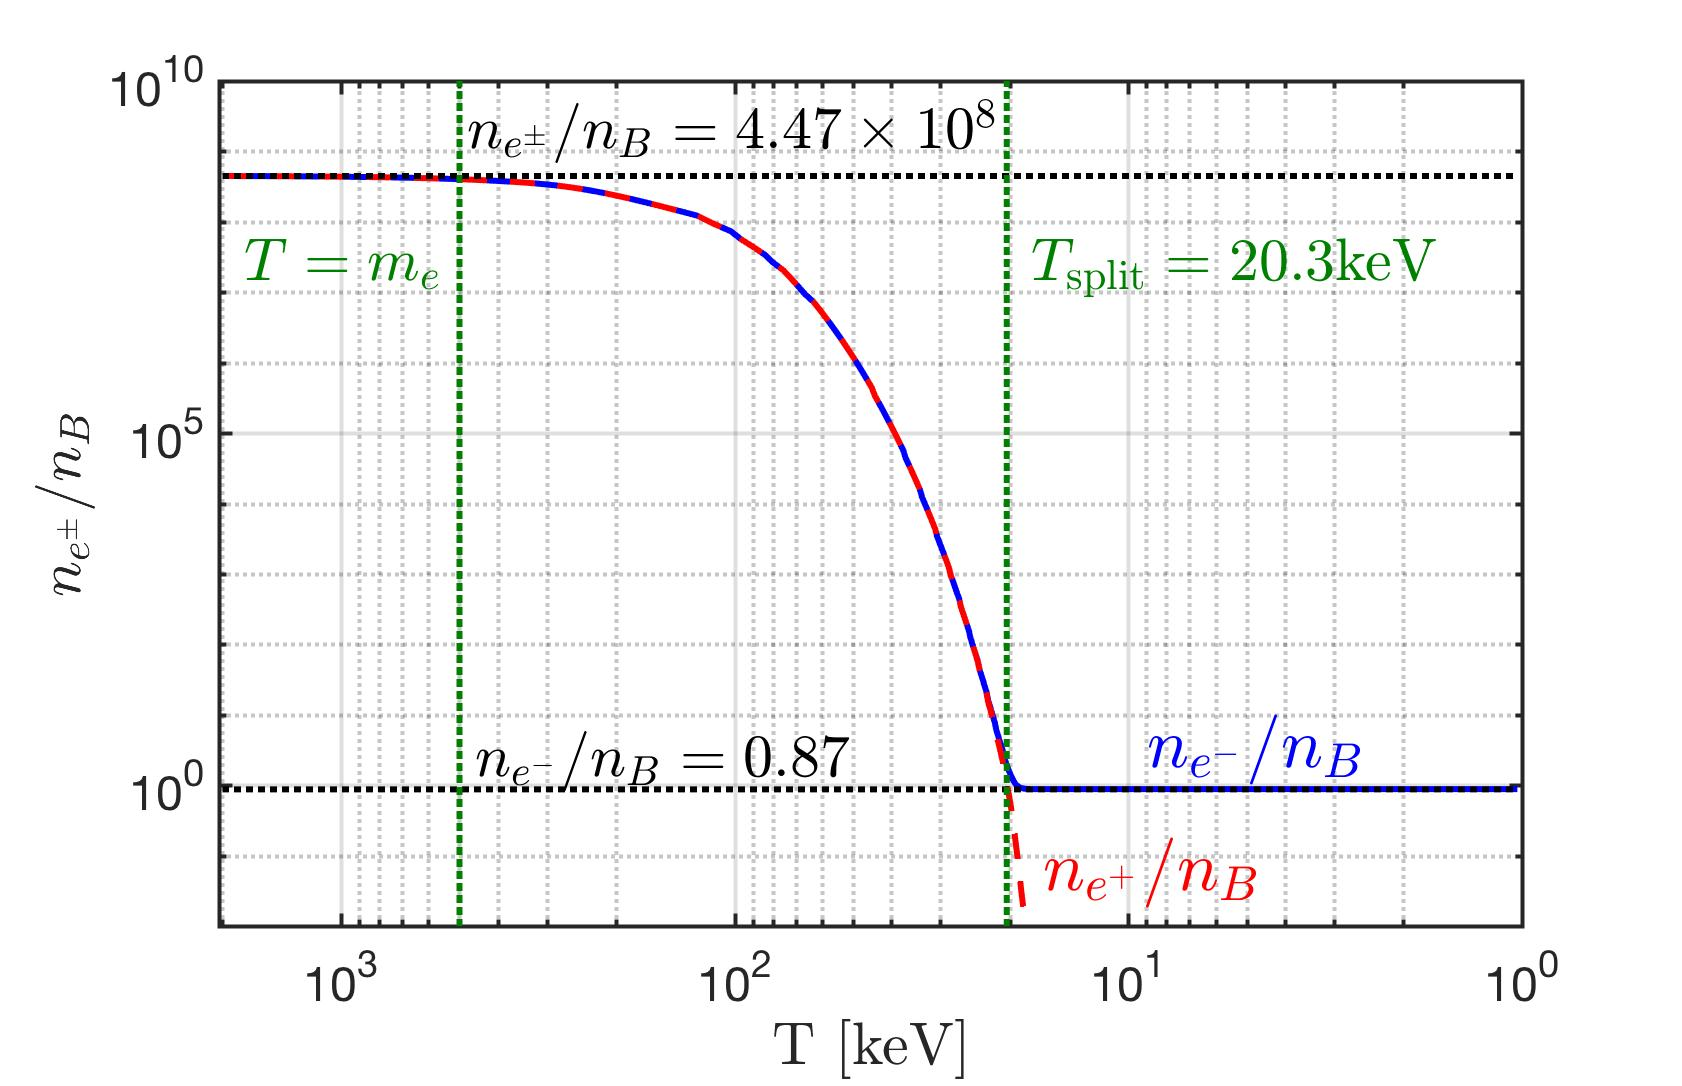
\includegraphics[width=0.8\textwidth]{plots/EEPlasmaDensityRatio_new.jpg}
    \caption{Electron $e^-$ and positron $e^+$ to baryon ratio $n_{e^{\pm}}/n_{B}$  as a function of photon temperature in the universe. See text for further details.}
    \label{fig:densityratio} 
\end{figure}
%%%%%%%%%%%%%%%%%%%%%%%%%%%%%%%%%%%%%%%

Large pre-recombination primordial fields could therefore lead to early universe baryon inhomogeneities which in turn would produce anisotropies in the cosmic microwave background (CMB)~\cite{jedamzik2013smallscale,abdalla2022cosmology}. Jedamzik and Pogosian~\cite{jedamzik2020relieving} propose further that the presence of ${\cal B}_{\rm PMF}\simeq0.1{\rm\ nG}$ could be sufficient to explain the Hubble tension. {\xblue We consider an entirely novel hypothesis that the primordial magnetization of the universe is driven by spin paramagnetism originating in the relatively dense electron-positron $e^{+}e^{-}$ plasma which reached about 100 million pairs per baryon at the pre-BBN temperature $T=200\keV$ (see: \rf{fig:densityratio}). These results were obtained using charge neutrality and the baryon to photon content (entropy) of the universe~\cite{rafelski2023short}.} 

{\xblue The electron-to-baryon ratio $n_{e^{-}}/n_{B}$ is shown in \rf{fig:densityratio} as the solid blue line which overlaps the positron-to-baryon ratio $n_{e^{+}}/n_{B}$, represented by the dashed red line, until the temperature drops below $T_{\rm split}=20.3\keV$ as the abundances of the two species diverge from one another.} The two vertical dashed green lines denote temperatures $T=m_{e}\simeq511\keV$ and $T_{\rm split}=20.3\keV$. {\xblue It is customary to show time as increasing from left to right which corresponds to a decreasing temperature. All figures in this paper will plot temperature as the $x$-axis scale.} The two horizontal black dashed lines denote the relativistic $T\gg m_e$ abundance of $n_{e^{\pm}}/n_{B}=4.47\times10^{8}$ and post-annihilation {\xblue abundance of  $n_{e^{-}}/n_{B}=0.87$. The deviation from unity in the post-annihilation abundance reflects the presence of bound neutrons in the baryon content.} Above temperature $T\simeq85\keV$, the $e^{+}e^{-}$ primordial plasma density exceeded that of the Sun's core density $n_{e}\simeq6\times10^{26}{\rm\ cm}^{-3}$~\cite{bahcall2001solar}. 

{\xblue Our analysis of the relativistic fermion partition function focuses} on the spin contribution to magnetization. {\xblue At $T\simeq200\keV$, due to very high $e^{+}e^{-}$ pair densities, we believe that spin paramagnetism is dominant over Landau orbital diamagnetism.} We show that magnetization is nonzero {\xblue even for a nearly symmetric particle-antiparticle gas as well as account for the matter-antimatter asymmetry present in the universe.} We further demonstrate that magnetization can spontaneously increase in strength near the IGMF upper limit seen in \req{igmf}. This is assisted by the fact that antiparticles $(e^{+})$ have the opposite sign of charge, and thus magnetic moment, compared to particles  $(e^{-})$. {\xblue Therefore in an $e^{+}e^{-}$ pair plasma, net magnetization can be associated with opposite spin orientations for particles and antiparticles without the accompaniment of} a net angular momentum in the volume considered. This is of course very different from the the matter dominated universe arising below $T\simeq20\keV$ which includes the current epoch.

%%%%%%%%%%%%%%%%%%%%%%%%%%%%%%%%%%%%%%%
\section{Electron-positron abundance}
\label{sec:abundance}
%%%%%%%%%%%%%%%%%%%%%%%%%%%%%%%%%%%%%%%
\noindent As the universe cooled below temperature $T=m_{e}$ (the electron mass), the thermal electron and positron comoving density {\xblue of $n_{e^{\pm}}/n_{B}=4.47\times10^{8}$} depleted falling over eight orders of magnitude. At $T_{\rm split}=20.3\keV$, the charged lepton asymmetry (mirrored by baryon asymmetry {\xblue and enforced by charge neutrality}) became evident {\xblue as the surviving excess electrons persisted while positrons vanished entirely from the particle inventory of the universe. Conversion of the dense $e^{+}e^{-}$ pair plasma into photons reheated the photon background~\cite{birrell2014relic} separating the photon and neutrino temperatures. The $e^{+}e^{-}$ annihilation and photon reheating period lasted no longer than an afternoon lunch break.} Because of charge neutrality, the post-annihilation comoving ratio $n_{e^{-}}/n_{B}=0.87$~\cite{rafelski2023short} is slightly offset from unity in~\rf{fig:densityratio} by the presence of bound neutrons in $\alpha$ particles and  other neutron containing light elements produced during BBN epoch. 

{\xblue To obtain a quantitative description of the above evolution, we study the bulk properties of the relativistic charged/magnetic gasses in a nearly homogeneous and isotropic primordial universe via} the thermal Fermi-Dirac or Bose distributions. {\xblue For matter $(\sigma=+1)$ and antimatter $(\sigma=-1)$ particles, a nonzero chemical potential $\mu_{\sigma}=\sigma\mu$ is caused by an imbalance of matter and antimatter. While the primordial electron-positron plasma era was overall charge neutral, there was a small asymmetry in the charged leptons from baryon asymmetry~\cite{fromerth2012quarkgluon,canetti2012matter} in the universe. Consideration of reactions such as $e^+e^-\leftrightarrow\gamma\gamma$ constrains the chemical potentials of electrons and positrons~\cite{elze1980relativistic} as 
\begin{align}
    \label{cpotential}
    \mu\equiv\mu_{e^{-}}=-\mu_{e^{+}}\,,\qquad
    \lambda\equiv\lambda_{e^{-}}=\lambda_{e^{+}}^{-1}=\exp\frac{\mu}{T}\,,
\end{align}
where $\lambda$ is the fugacity of the system.} 

{\xblue During the $e^{+}e^{-}$ plasma epoch, the density changed dramatically over time (see: \rf{fig:densityratio}) changing the chemical potential in turn. We can then parameterize the chemical potential of the $e^{+}e^{-}$ plasma as a function of temperature $\mu\rightarrow\mu(T)$ via the charge neutrality of the universe which implies}
\begin{align}
    \label{chargeneutrality}
    n_{p}=n_{e^{-}}-n_{e^{+}}=\frac{1}{V}\lambda\frac{\partial}{\partial\lambda}\ln{\cal Z}_{e^{+}e^{-}}\,.
\end{align}
{\xblue In \req{chargeneutrality}, $n_{p}$ is the observed total number density of protons in all baryon species. The parameter $V$ relays the proper volume under consideration and $\ln{\cal Z}_{e^{+}e^{-}}$ is the partition function for the electron-positron gas. The chemical potential defined in \req{cpotential} is obtained from the requirement that the positive charge of baryons (protons, $\alpha$ particles, light nuclei produced after BBN) is exactly and locally compensated by a tiny net excess of electrons over positrons.}

{\xblue The abundance of baryons is itself fixed by the known abundance relative to photons~\cite{workman2022pdg} and we employed the contemporary recommended value $n_B/n_\gamma=6.09\times 10^{-10}$.} The resulting chemical potential  needs to be evaluated carefully to obtain the behavior near to $T_{\rm split}=20.3\keV$ where the relatively {\xblue small value of chemical potential $\mu$} rises rises rapidly so that positrons vanish from the particle inventory of the universe while nearly one electron per baryon remains. The detailed solution of this problem is found in Refs.\;\cite{fromerth2012quarkgluon,rafelski2023short} leading to the results shown in \rf{fig:densityratio}. These results are obtained allowing for Fermi-Dirac and Bose statistics, however it is often numerically sufficient to consider the Boltzmann distribution limit.

In the presence of a magnetic field ${\cal B}$ there is some modification of the usual relativistic fermion partition function which is now given  by
\begin{align}
    \label{partition}
    \ln{\cal Z}_{e^{+}e^{-}}=\frac{e{\cal B}V}{(2\pi)^{2}}\sum_{\sigma}^{\pm}\sum_{s}^{\pm}\sum_{n=0}^{\infty}\int_{-\infty}^{\infty}{\rm d}p_{z}\left[\ln\left(1+\lambda_{\sigma}\xi_{s}e^{-E_{n}^{s}/T}\right)\right]\,,\qquad\Upsilon_{\sigma}^{s}=\lambda_{\sigma}\xi_{s}=\exp{\frac{\mu_{\sigma}+\eta_{s}}{T}}\,,
\end{align}
{\xblue with electric charge $e\equiv q_{e^{+}}=-q_{e^{-}}$.} The index $\sigma$ in \req{partition} is a sum over electron and positron states while $s$ is a sum over polarizations. Since we are interested in small asymmetries (e.g. baryon excess over antibaryons, one spin polarization over another) we introduce the generalized particle fugacity $\Upsilon_{\sigma}^{s}$ as the product of:
\begin{itemize}
    \item[a.] Chemical fugacity $\lambda_{\sigma}$
    \item[b.] Spin fugacity $\xi_{s}$
\end{itemize}
The chemical fugacity $\lambda_{\sigma}$ {\xblue (defined in \req{cpotential} above) describes deformation of the Fermi-Dirac distribution due to nonzero chemical potential $\mu$.} An imbalance in electrons and positrons leads {\xblue as discussed earlier} to a nonzero particle chemical potential $\mu\neq0$. We then introduce a novel spin fugacity $\xi_{s}$ and spin potential $\eta_{s}=s\eta$. {\xblue We propose the spin potential follows analogous expressions as seen in \req{cpotential} obeying
\begin{align}
    \label{spotential}
    \eta\equiv\eta_{+}=-\eta_{-}\,,\qquad
    \xi\equiv\xi_{+}=\xi_{-}^{-1}= \exp{\frac{\eta}{T}}\,.
\end{align}

An imbalance in spin polarization within a region of volume $V$ results in a nonzero spin potential $\eta\neq0$. Conveniently since antiparticles have opposite sign of charge and magnetic moment, the same magnetic moment is associated with opposite spin orientation for particles and antiparticles independent of degree of spin-magnetization. A completely particle-antiparticle symmetric magnetized plasma will have therefore zero total spin angular momentum and zero spin potential $\eta=0$. This is of course very different from situation in the matter dominated universe of the current epoch.}

%%%%%%%%%%%%%%%%%%%%%%%%%%%%%%%%%%%%%%%
\section{Primordial paramagnetism }
\label{sec:fugacity}
%%%%%%%%%%%%%%%%%%%%%%%%%%%%%%%%%%%%%%%
\noindent
As the universe undergoes isotropic expansion, the temperature decreases as 
\begin{align}
    \label{tscale}
    T(t)=T_{0}\frac{a_{0}}{a(t)}\rightarrow T(z)=T_{0}(1+z)\,,
\end{align}
where $a(t)$ is the scale factor defined by the FLRW metric~\cite{weinberg1972gravitation} and $z$ is the redshift. The comoving temperature $T_{0}$ is given by the present day temperature of the CMB,  contemporary scale factor $a_{0}=1$. Within a homogeneous magnetic domain, the magnetic field varies~\cite{durrer2013cosmological} over cosmic expansion as
\begin{align}
    \label{bscale}
    {\cal B}(t)={\cal B}_{0}\frac{a_{0}^{2}}{a^{2}(t)}\rightarrow{\cal B}(z)={\cal B}_{0}\left(1+z\right)^{2}\,,
\end{align}
where ${\cal B}_{0}$ is the comoving value of the magnetic field obtained from the contemporary value of the magnetic field today  given in \req{igmf}. Non-primordial magnetic fields (which are generated through other mechanisms  such as dynamo or astrophysical sources) do not follow this scaling~\cite{pomakov2022redshift}. The presence of matter and late universe structure formation also  contaminates the primordial field evolution in \req{bscale}. It is only in deep intergalactic space where primordial fields remain preserved and comoving over cosmic time.

From \req{tscale} and \req{bscale} emerges a natural ratio of interest here which is conserved over cosmic expansion 
\begin{align}
    \label{tbscale}
    b \equiv\frac{e{\cal B}(t)}{T^{2}(t)}=\frac{e{\cal B}_{0}}{T_{0}^{2}}\equiv b_0={\rm\ const.}\qquad10^{-3}>b_{0}>10^{-11}\,,
\end{align}
given in natural units ($c=\hbar=k_{B}=1$). We computed the bounds for this cosmic magnetic scale ratio by using the present day observations given by \req{igmf} and the present CMB temperature $T_{0}=2.7{\rm\ K}\simeq2.3\times10^{-4}\eV$~\cite{aghanim2018planck}.

To evaluate paramagnetic properties of the $e^-e^+$-pair plasma We take inspiration from Ch. 9 of Melrose's treatise on magnetized plasmas~\cite{melrose2008quantum}. We focus  on the bulk properties of thermalized plasmas in (near) equilibrium. In considering $e^{+}e^{-}$-pair plasma, we introduce the microscopic energy of the charged $q=\pm e$ relativistic fermion within a homogeneous ($z$-direction) magnetic field~\cite{steinmetz2018magnetic}. The energy eigenvalue is given by
\begin{align}
    \label{kgp}
    E^{\pm}_{n}(p_{z},{\cal B})=\sqrt{m_{e}^{2}+p_{z}^{2}+e{\cal B}\left(2n+1\mp\frac{g}{2}\right)}\,,\qquad n\in0,1,2,\ldots
\end{align}
where $p_{z}$ is the momentum parallel to the field axis and $n$ is the Landau orbital quantum number. The subscript $\pm$ refers to the spin polarization along the field axis: parallel $(+)$ or anti-parallel $(-)$ (AND OPPOSITE FOR ANTIPARTICLES???). The parameter $g$ is the gyro-magnetic ($g$-factor) of the particle. We rearrange \req{kgp} by pulling the spin dependency and the ground state Landau orbital into the mass writing
\begin{align}
    \label{effmass}
    E^{\pm}_{n}={\tilde m}_{\pm}\sqrt{1+\frac{p_{z}^{2}}{{\tilde m}_{\pm}^{2}}+\frac{2e{\cal B}n}{{\tilde m}_{\pm}^{2}}}\,,\qquad {\tilde m}_{\pm}^{2}=m_{e}^{2}+q{\cal B}\left(1\mp\frac{g}{2}\right)\,,
\end{align}
where we introduced the effective polarized mass ${\tilde m}_{\pm}$ which is distinct for each spin alignment and is a function of magnetic field strength ${\cal B}$. The effective polarized mass ${\tilde m}_{\pm}$ allows us to describe the $e^{+}e^{-}$ plasma with the spin effects almost wholly separated from the Landau characteristics of the gas when considering plasma thermodynamic properties.
 The electron-positron number density ratio relative to the baryon number density in the temperature range $2000\keV>T>20\keV$the  $e^{+}e^{-}$ results we have shown in~\rf{fig:densityratio},    . 

In presence of magnetic field in Boltzmann approximation the charge neutrality condition \req{chargeneutrality} becomes
\begin{align}
    \label{chem}
    \sinh{\frac{\mu}{T}}=n_{p}\frac{\pi^{2}}{T^{3}}\left[\sum_{s}^{\pm}\xi_{s}\left(x_{s}^{2}K_{2}(x_{s})+\frac{b_{0}}{2}x_{s}K_{1}(x_{s})+\frac{b_{0}^{2}}{12}K_{0}(x_{s})\right)\right]^{-1}\,.
\end{align}
\req{chem} is fully determined by the right-hand-side expression if the spin fugacity is set to unity $\xi=1$ implying an equal number of polarizations both parallel and anti-parallel to the external field. 

In general however, an additional physical constraint is required as the chemical $\mu$ and spin $\eta$ potentials have mutual dependency. We note that such a constraint is likely related to the total angular momentum of the considered volume and does not necessarily imply that spin polarizations must be balanced within a single species when the orbital and spin momentum of all species in the plasma are taken into account.

SOME MORE REFERENCES OR/AND DETAIL\\

Since our arguments address the temperature interval  where for the  $e^{+}e^{-}$-pair plasma effects of quantum Fermi statistics are relatively small we employ throughout the Boltzmann approximation. However, we extrapolate our results for presentation completeness up to $T\simeq 4m$. In general modifications due to quantum statistical phase space reduction for fermions are expected to reduce by about 20\% such extrapolated results and perhaps by  a lesser amount the relative values. We continue to search for semi-analytical solutions allowing spin ferromagnetism for Fermi statistics in relativistic  $e^{+}e^{-}$-pair abundance akin to the Boltzmann solution here offered. 

We proceed now with the Boltzmann approximation for the limit where $T\lesssim m_e$. The Euler-Maclaurin formula~\cite{abramowitz1988handbook} is used to convert the summation over Landau levels into an integration. The resulting partition function (after truncation of the error remainder) can then be written in terms of modified Bessel $K$ functions~\cite{abramowitz1988handbook,letessier2002hadrons} of the second kind, yielding
\begin{align}
    \label{boltzmann}
    \ln{\cal Z}_{e^{+}e^{-}}\simeq\frac{T^{3}V}{2\pi^{2}}\left[2\cosh{\frac{\mu}{T}}\right]\sum_{s}^{\pm}\xi_{s}\left(x_{s}^{2}K_{2}(x_{s})+\frac{b_{0}}{2}x_{s}K_{1}(x_{s})+\frac{b_{0}^{2}}{12}K_{0}(x_{s})\right)\,,\\
    \label{xfunc}
    2\cosh{\frac{\mu}{T}}=\lambda+\lambda^{-1}\,,\qquad
    x_{\pm}=\frac{{\tilde m}_{\pm}}{T}=\sqrt{\frac{m_{e}^{2}}{T^{2}}+b_{0}\left(1\mp\frac{g}{2}\right)}\,.
\end{align}
The latter two terms in \req{boltzmann} (proportional to $b_{0}K_{1}$ and $b_{0}^{2}K_{0}$) are the uniquely magnetic terms present (containing both paramagnetic and diamagnetic influences) in the partition function while the $K_{2}$ term is present for the relativistic free Fermi gas~\cite{greiner2012thermodynamics}. As the Bessel $K$ functions are evaluated as functions of $x_{\pm}$ in \req{xfunc}, the \lq\lq free\rq\rq\ part of the partition $K_{2}$ is still subject to spin magnetization effects.
%%%%%%%%%%%%%%%%%%%%%%%%%%%%%%%%%%%%%%%
\section{Electron-positron magnetization}
\label{sec:magnetization}
\noindent The magnetization of the $e^{+}e^{-}$ plasma described by the partition function in \req{boltzmann} can be written as
\begin{align}
    \label{defmagetization}
    {\cal M}\equiv\frac{T}{V}\frac{\partial}{\partial{\cal B}}\ln{{\cal Z}_{e^{+}e^{-}}} = \frac{T}{V}\left(\frac{\partial b_{0}}{\partial{\cal B}}\right)\frac{\partial}{\partial b_{0}}\ln{{\cal Z}_{e^{+}e^{-}}}\,,\qquad\frac{\partial b_{0}}{\partial{\cal B}}=\frac{q}{T^{2}}\,.
\end{align}
Magnetization arising from other components in the cosmic gas (protons, neutrinos, etc.) could in principle also be included. In the context of MHD, primordial magnetogenesis from neutrino interactions in the electron-positron epoch was considered in~\cite{perrone2021neutrinoelectron}. We introduce dimensionless units for magnetization by defining the critical field
\begin{align}
    {\cal B}_{C}\equiv\frac{m_{e}^{2}}{q}\,,\qquad{\overline{\cal M}}\equiv\frac{\cal M}{{\cal B}_{C}}\,.
\end{align}

%%%%%%%%%%%%%%%%%%%%%%%%%%%%%%%%%%%%%%%
\begin{figure}[ht]
    \centering
    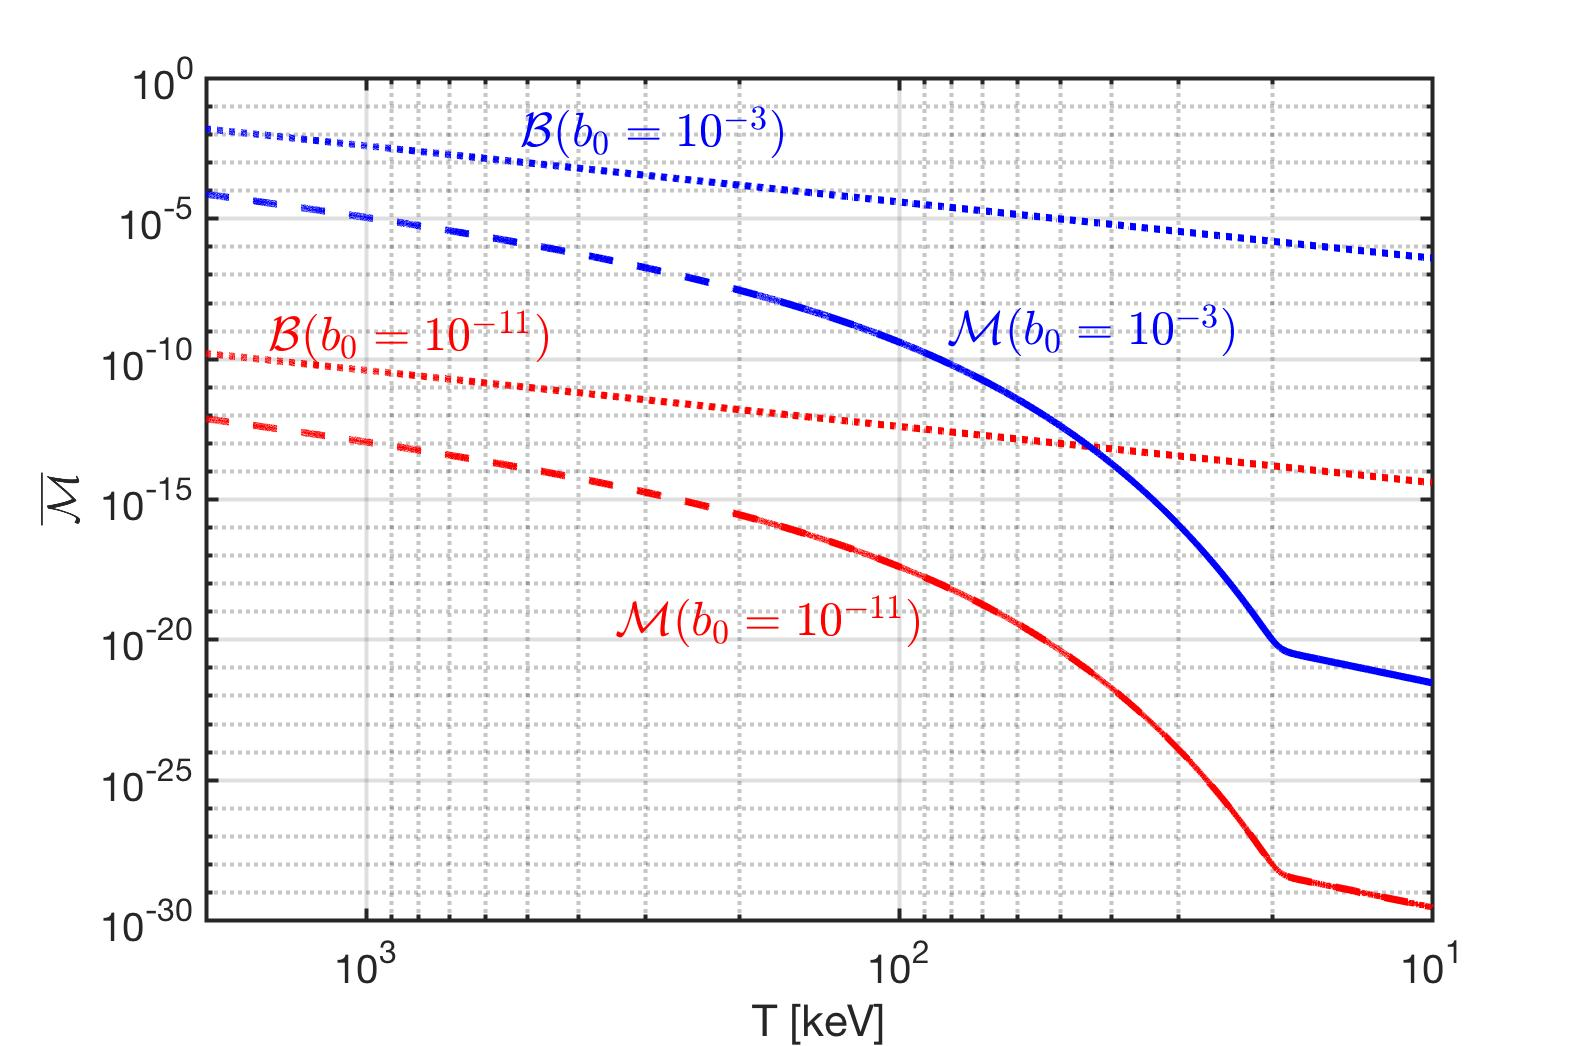
\includegraphics[width=0.8\textwidth]{Magnetization_Hc_new002.jpg}
    \caption{The magnetization ${\cal M}$, with $g=2$, of the primordial $e^{+}e^{-}$ plasma is plotted as a function of temperature. The lower (solid red) and upper (solid blue) bounds for cosmic magnetic scale $b_{0}$ are included. The external magnetic field strength ${\cal B}/{\cal B}_{C}$ is also plotted in for lower (dashed red) and upper (dashed blue) bounds. The spin fugacity is set to unity $\xi=1$.}
    \label{fig:magnet} 
\end{figure}
%%%%%%%%%%%%%%%%%%%%%%%%%%%%%%%%%%%%%%%

%%%%%%%%%%%%%%%%%%%%%%%%%%%%%%%%%%%%%%%
\begin{figure}[ht]
    \centering
    \begin{subfigure}{0.49\textwidth}
        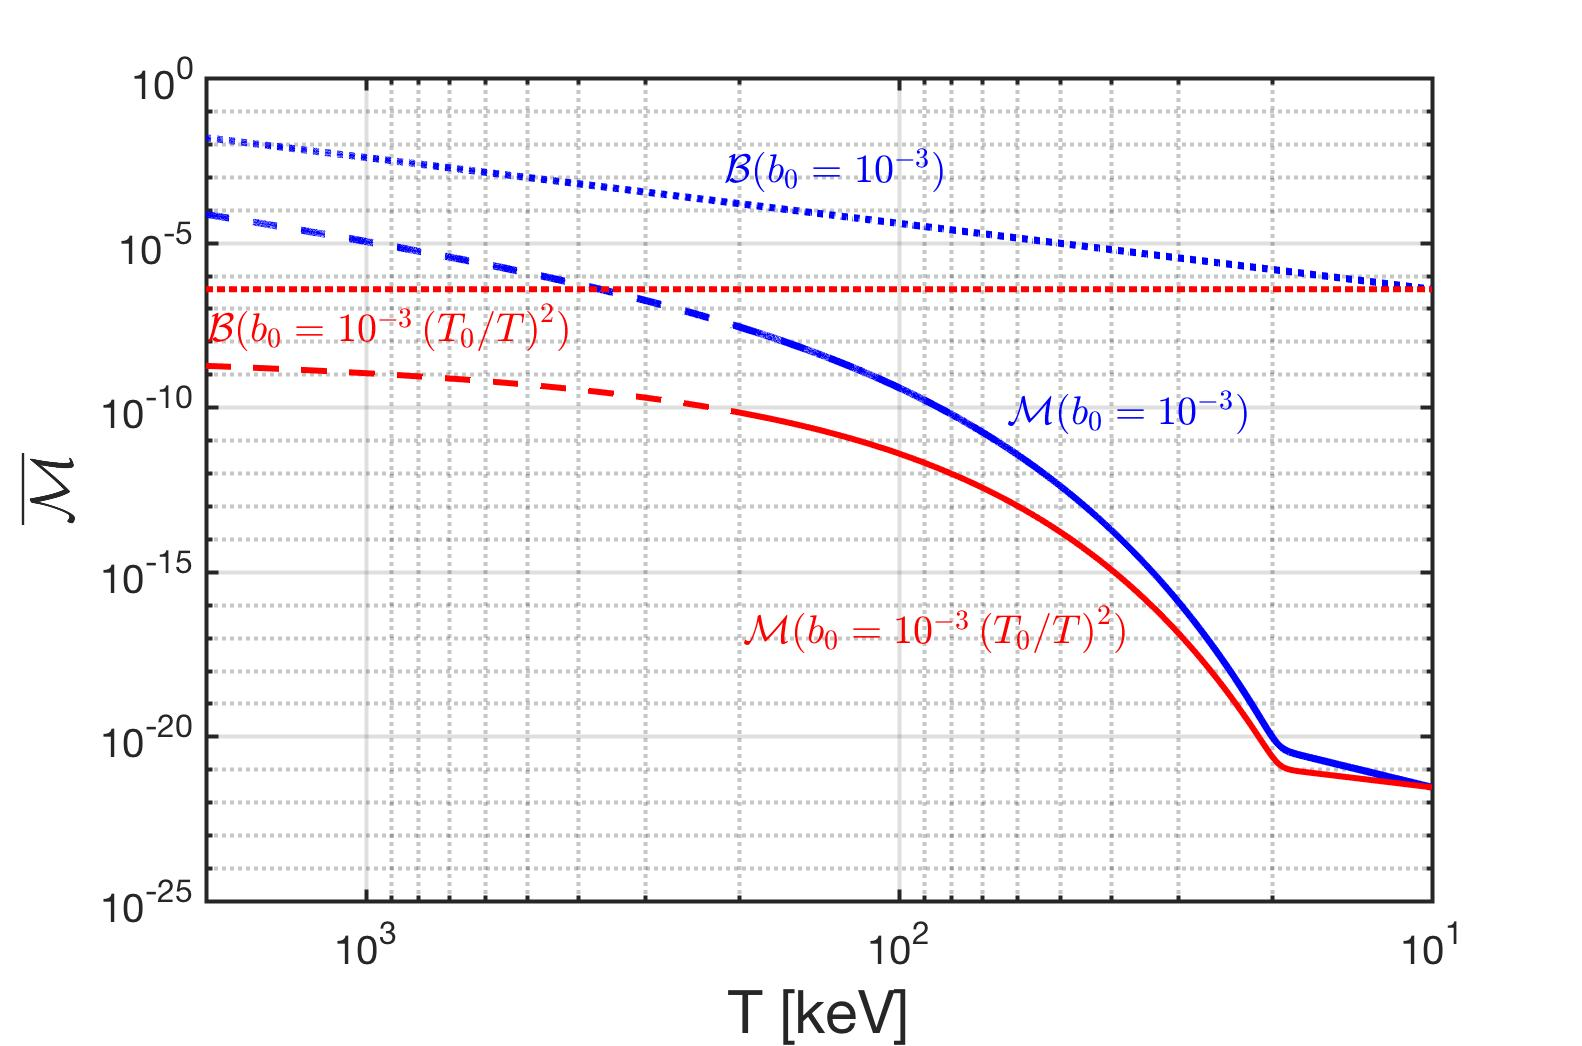
\includegraphics[width=\textwidth]{Magnetization_Hc_constant.jpg}
    \end{subfigure}
    \hfill
    \begin{subfigure}{0.49\textwidth}
        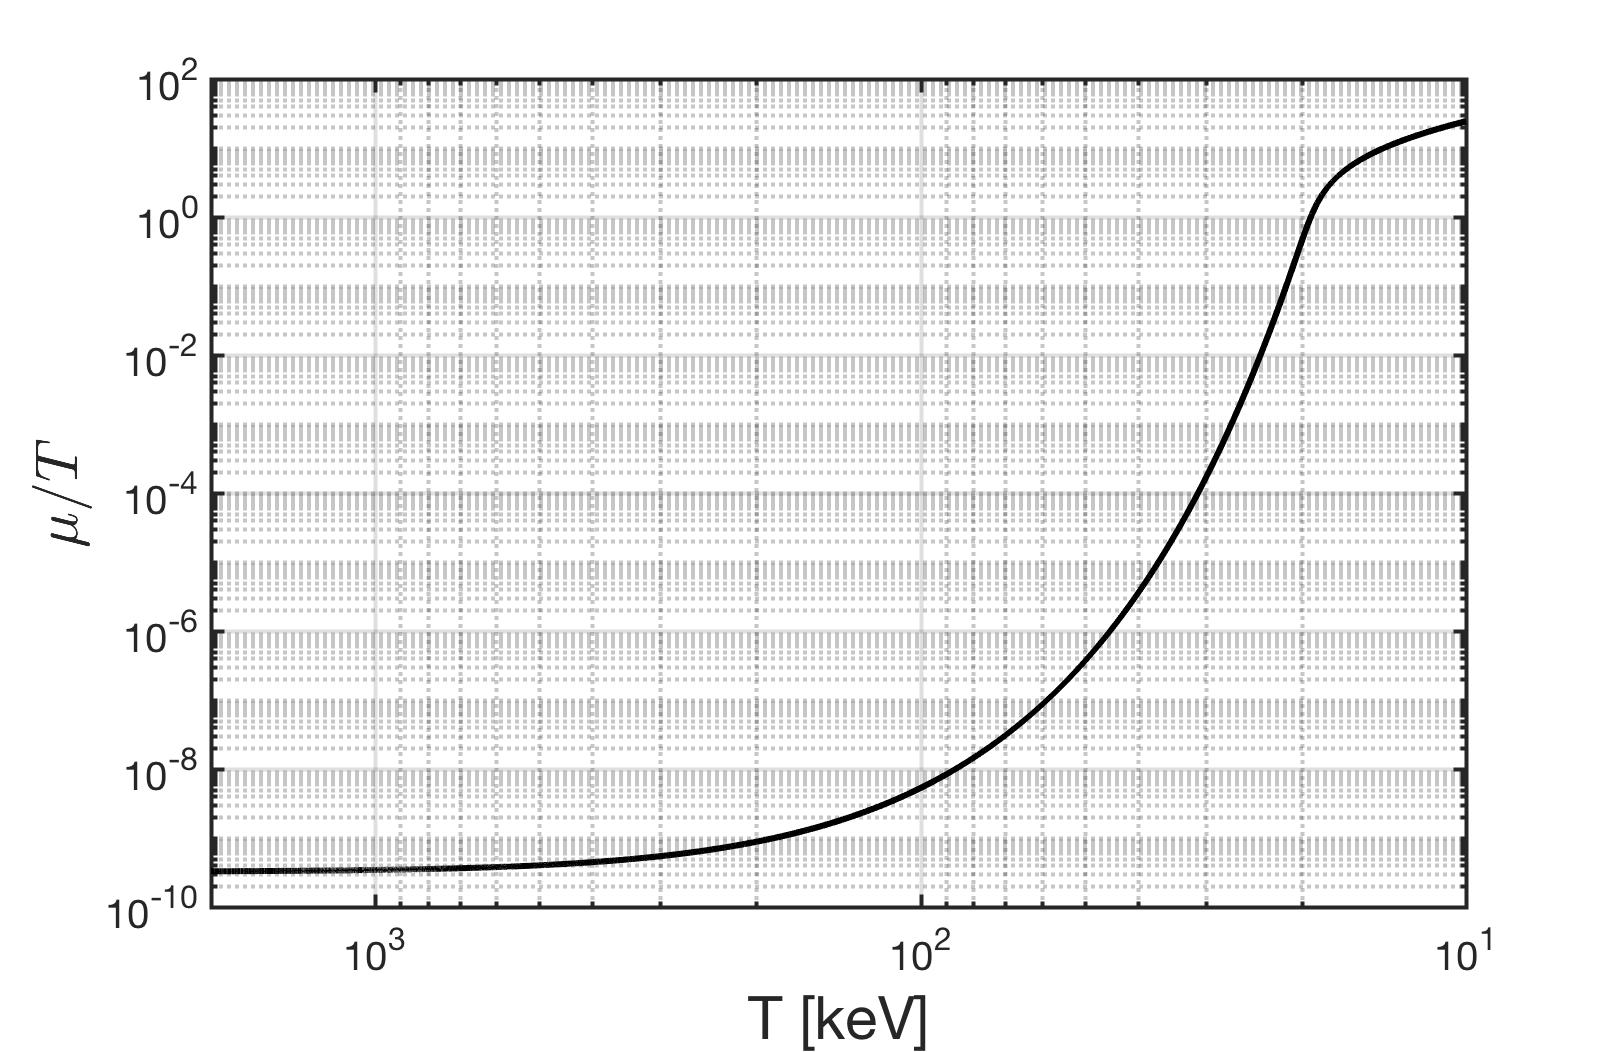
\includegraphics[width=\textwidth]{ChemicalPotential_new.jpg}
    \end{subfigure}
    \caption{(left) The magnetization ${\cal M}$, with $g=2$, is plotted for the $b_{0}=10^{-3}$ case (solid blue) and the constant magnetic field $b_{0}=10^{-3}(T_{0}/T)^{2}$ case (solid red) where the comoving reference temperature is $T_{0}=10\keV$. The external magnetic field strength is plotted for the conserved flux case (dashed blue) and the constant field case (dashed red). (right) The chemical potential over temperature $\mu/T$ is plotted as a function of temperature with magnetic field $b_{0}=0$ and spin potential $\eta=0$ set to zero.}
    \label{fig:paireffect}
\end{figure}
%%%%%%%%%%%%%%%%%%%%%%%%%%%%%%%%%%%%%%%

The scale ${\cal B}_{C}$ is where electromagnetism is expected to become subject to non-linear effects, though luckily in our regime of interest, electrodynamics should be linear. We note however that the upper bounds of IGMFs in \req{igmf} (with $b_{0}=10^{-3}$; see \req{tbscale}) brings us to within $1\%$ of that limit for the external field strength in the temperature range considered. The total magnetization ${\cal M}$ can be broken into the sum of spin parallel ${\cal M}_{+}$ and spin anti-parallel ${\cal M}_{-}$ magnetization. We note that the expression for the magnetization simplifies significantly for $g=2$ which is the \lq\lq cusp\rq\rq\ gyro-magnetic factor~\cite{rafelski2022study} for Dirac particles. For illustration, the $g=2$ magnetization from \req{defmagetization} is then
\begin{align}
    \label{g2magplus}
    {\overline{\cal M}}_{+}&=\frac{q^{2}}{\pi^{2}}\frac{T^{2}}{m_{e}^{2}}\xi\cosh{\frac{\mu}{T}}\left[\frac{1}{2}x_{+}K_{1}(x_{+})+\frac{b_{0}}{6}K_{0}(x_{+})\right]\,,\qquad x_{+}=\frac{m_{e}}{T}\,,\\
    \label{g2magminus}
    -{\overline{\cal M}}_{-}&=\frac{q^{2}}{\pi^{2}}\frac{T^{2}}{m_{e}^{2}}\xi^{-1}\cosh{\frac{\mu}{T}}\left[\left(\frac{1}{2}+\frac{b_{0}^{2}}{12x_{-}^{2}}\right)x_{-}K_{1}(x_{-})+\frac{b_{0}}{3}K_{0}(x_{-})\right]\,,\qquad x_{-}=\sqrt{\frac{m_{e}^{2}}{T^{2}}+2b_{0}}\,.
\end{align}
As the $g$-factor of the electron is only slightly above two at $g\simeq2.00232$~\cite{tiesinga2021codata}, the above two expressions for ${\overline{\cal M}}_{+}$ and ${\overline{\cal M}}_{-}$ are only modified by a small amount because of anomalous magnetic moment (AMM). The influence of AMM would be more relevant for the magnetization of baryon gasses since the $g$-factor for protons $(g\approx5.6)$ and neutrons $(g\approx3.8)$ are substantially different from $g=2$.

In \rf{fig:magnet}, we plot the magnetization as given by \req{g2magplus} and \req{g2magminus} with the spin potential set to unity $\xi=1$. We see that the $e^{+}e^{-}$ plasma is overall paramagnetic and yields a positive overall magnetization which is contrary to the traditional assumption that matter-antimatter plasmas lack significant magnetic responses of their own in the bulk. With that said, the magnetization never exceeds the external field under the parameters considered which shows a lack of ferromagnetic behavior. As the universe cooled, the dropping magnetization slowed at $T_{\rm split}=20.3\keV$ where positrons vanished. Thereafter the remaining electrons density $n_{e^{-}}$ only diluted with cosmic expansion.

%%%%%%%%%%%%%%%%%%%%%%%%%%%%%%%%%%%%%%%
\begin{figure}[ht]
    \centering
    \begin{subfigure}[b]{0.49\textwidth}
        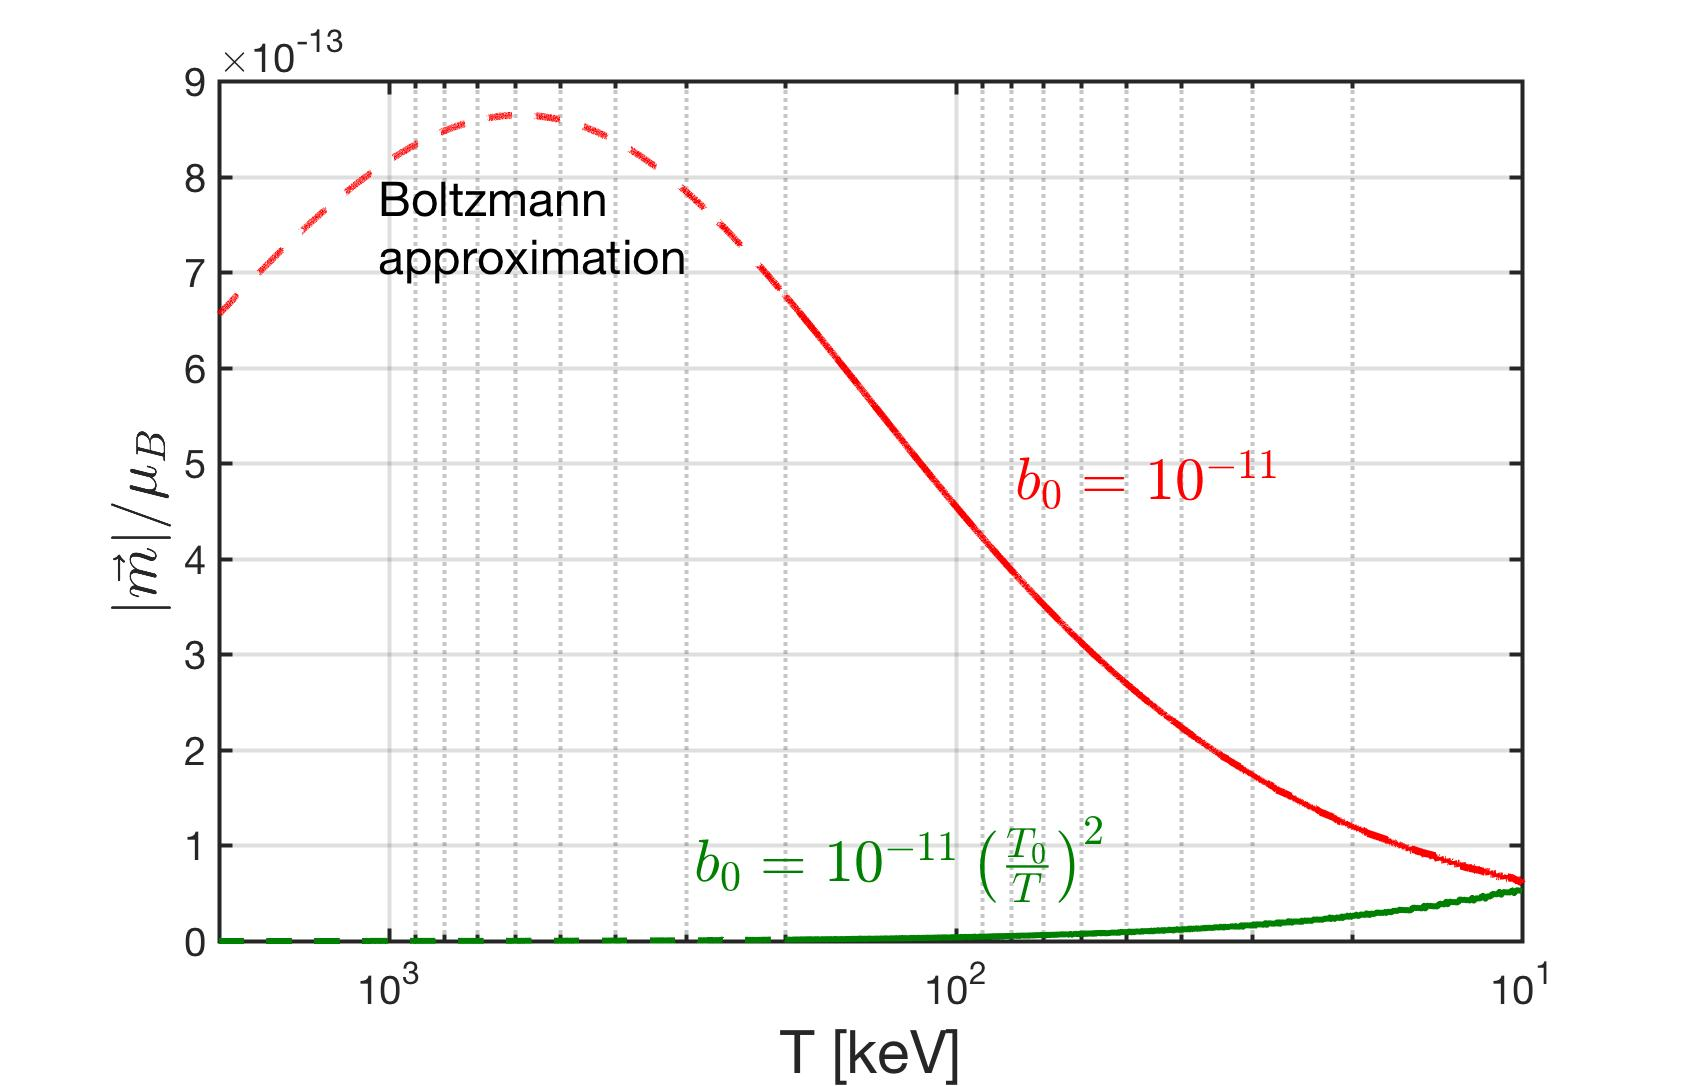
\includegraphics[width=\textwidth]{NewMagnetizationDensity001_Boltz.jpg}
    \end{subfigure}
    \hfill
    \begin{subfigure}[b]{0.49\textwidth}
        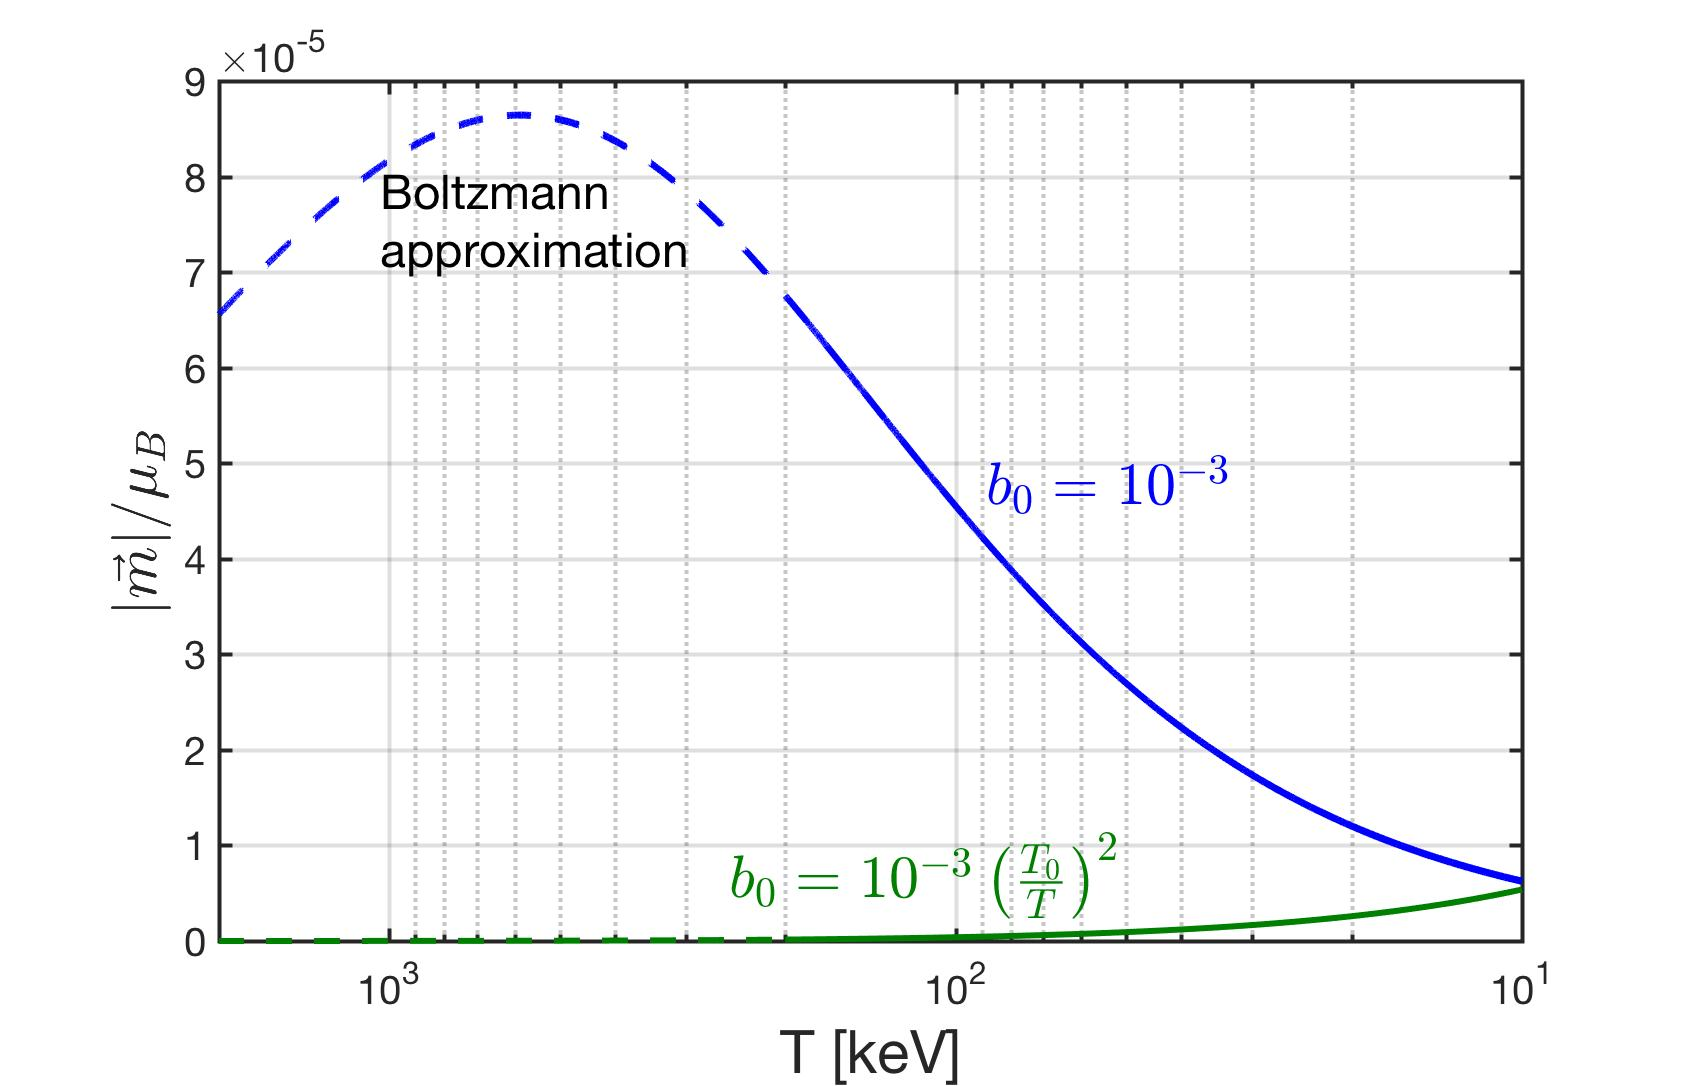
\includegraphics[width=\textwidth]{NewMagnetizationDensity002_Boltz.jpg}
    \end{subfigure}
    \caption{The magnetic moment per lepton $\langle\vec{m}\rangle_{z}$ along the field axis is plotted for (left) $b_{0}=10^{-11}$ and (right) $b_{0}=10^{-3}$ using the Boltzmann approximation (dashed black) and the Fermi-Dirac distribution (left: solid red; right: solid blue). Both figures display the constant magnetic field case (solid green) with the comoving value chosen at temperature $T_{0}~=~10\keV$.}
    \label{fig:momentperlepton}
\end{figure}
%%%%%%%%%%%%%%%%%%%%%%%%%%%%%%%%%%%%%%%

Despite the relatively large magnetization seen in \rf{fig:magnet}, the average contribution per lepton is only a small fraction of its overall magnetic moment. Specifically, the magnetization regime we are in is described by
\begin{align}
    \label{fractionalmagnetization}
    {\cal M}V\ll\mu_{B}(N_{e^{+}}+N_{e^{-}})\,,\qquad\mu_{B}=\frac{q}{2m}\,,
\end{align}
where $\mu_{B}$ is the Bohr magneton and $N=nV$ is the total particle number in the proper volume. To better demonstrate this, we define the average magnetic moment per lepton given by along the field ($z$-direction) axis as
\begin{align}
    \label{momentperlepton}
    \langle\vec{m}\rangle_{z}\equiv\frac{{\cal M}}{n_{e^{-}}+n_{e^{+}}}\,,\qquad\langle\vec{m}\rangle_{x}=\langle\vec{m}\rangle_{y}=0\,.
\end{align}
From the spin eigen-states, we expect the transverse expectation values to be zero. The quantity given in \req{momentperlepton} gives us an insight into the microscopic response of the plasma which we will use below.

A curious feature of \rf{fig:magnet} is that the magnetization increases as a function of temperature. This is contrary to most systems which lose their magnetization at higher temperatures because of the disordering influence of thermal heat~\cite{huang1991statistical}. A standard feature of paramagnetic systems (Curie's law) is that the susceptibility of the material is suppressed as temperature increases, so it is natural ask: Why doesn't this occur for the primordial $e^{+}e^{-}$ plasma?

There are two reasons:
\begin{itemize}
    \item[a.] As discussed in \rsec{sec:abundance}, the late $e^{+}e^{-}$ plasma saw its density decrease by a factor of $10^{9}$ as the majority of the gas annihilated leaving behind only a small residual quantity of electrons. As we travel into the distance past, the density of electrons $n_{e^{-}}$ and positrons $n_{e^{+}}$ increases by an enormous extent therefore enhancing the overall magnetization through quantity. This is shown in \rf{fig:paireffect} (left) which compares the magnetization of the gas with conserved magnetic flux $b_{0}={\rm\ const}$ and a constant field $b_{0}\propto1/T^{2}$. If the magnetic field is constant, we see the parameter responsible for magnetization at high temperatures is the pair density. In \rf{fig:paireffect} (right) we plot the chemical potential $\mu/T$ which characterizes the importance of the charged lepton asymmetry as a function of temperature. As an aside, we only plotted the $b_{0}=0$ case as the magnetic field did not visibly influence $\mu/T$ in the regime considered.
    \item[b.] The conservation of magnetic flux, as described in \req{bscale}, through comoving surfaces for the external field ensures that as we travel into the past, the magnetic field increases which enhances the overall magnetization of the gas. This phenomenon is seen in \rf{fig:paireffect} as the difference between the blue and red curves. However, a more striking visualization of this is plotted in \rf{fig:momentperlepton} where the average magnetic moment $\langle\vec{m}\rangle_{z}$ defined in \req{momentperlepton} displays how essential the external field is on the per lepton magnetization. The average magnetic moment per lepton is suppressed at higher temperatures (as expected for Curie law-like magnetization) if the field strength is held constant. A small difference is seen between the full Fermi distribution analysis and the Boltzmann approximation used in this work.
\end{itemize}

%%%%%%%%%%%%%%%%%%%%%%%%%%%%%%%%%%%%%%%
\section{Spin potential and ferromagnetism}
\label{sec:spin}
\noindent Up to this point, we have neglected the impact that a nonzero spin potential $\eta\neq0$ (and thus $\xi\neq1$) would have on the primordial $e^{+}e^{-}$ plasma. In the limit the cosmic magnetic scale (and thus external magnetic field) goes to zero, the magnetization given in \req{g2magplus} and \req{g2magminus} is entirely controlled by the spin fugacity $\xi$ asymmetry generated by the spin potential $\eta$ yielding
\begin{align}
    \lim_{b_{0}\rightarrow0}{\overline{\cal M}}=\frac{q^{2}}{\pi^{2}}\frac{T^{2}}{m_{e}^{2}}\sinh{\frac{\eta}{T}}\cosh{\frac{\mu}{T}}\left[\frac{m_{e}}{T}K_{1}\left(\frac{m_{e}}{T}\right)\right]\,,\qquad2\sinh{\frac{\eta}{T}}=\xi-\xi^{-1}\,.
\end{align}
Therefore, we can understand the spin potential as a kind of ferromagnetic influence on the primordial gas which allows for magnetization even in the absence of external magnetic fields. As $\sinh{\eta/T}$ is an odd function, the sign of $\eta$ also controls the alignment of the magnetization. In general, $\eta=\eta(\mu,T)$ is a function of the chemical potential and temperature. As discussed in \rsec{sec:fugacity}, the two potentials are mutually related likely would need be simultaneously solved. We will return to the topic of spin potential constraints under separate cover.
%%%%%%%%%%%%%%%%%%%%%%%%%%%%%%%%%%%%%%%
\begin{figure}[ht]
    \centering
    \begin{subfigure}[b]{0.49\textwidth}
        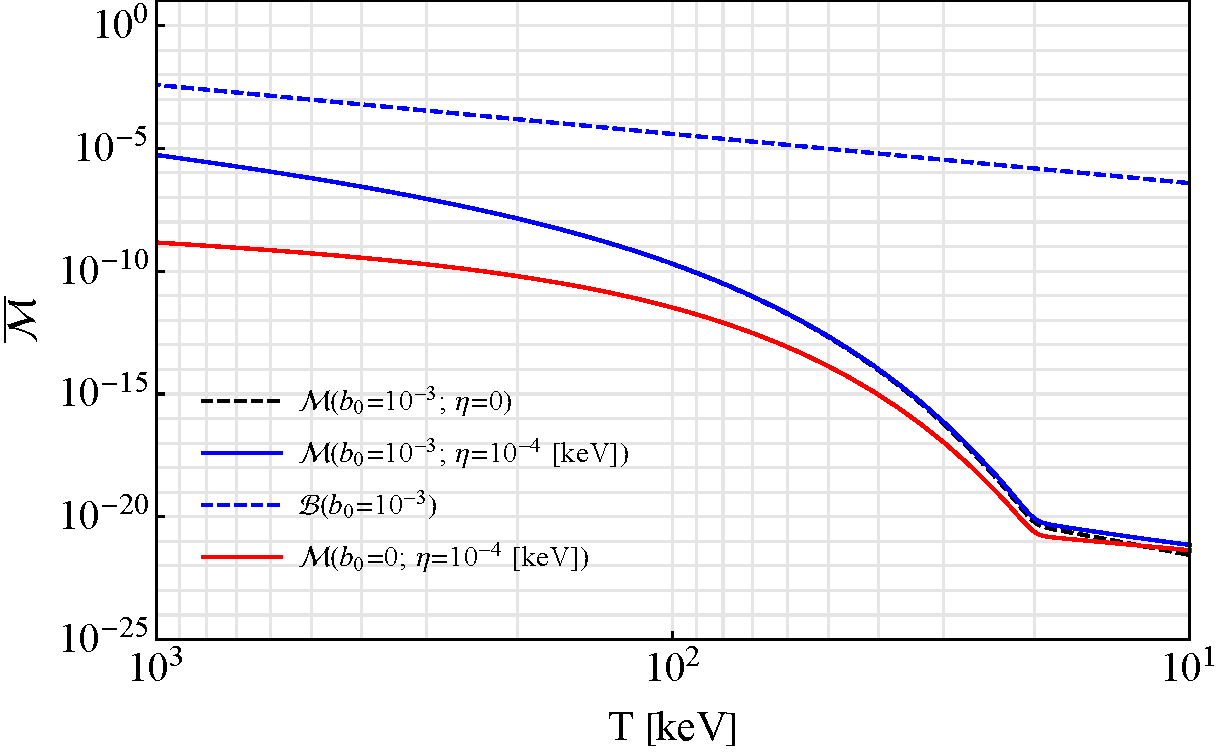
\includegraphics[width=\textwidth]{SpinLowFugacity.pdf}
    \end{subfigure}
    \hfill
    \begin{subfigure}[b]{0.49\textwidth}
        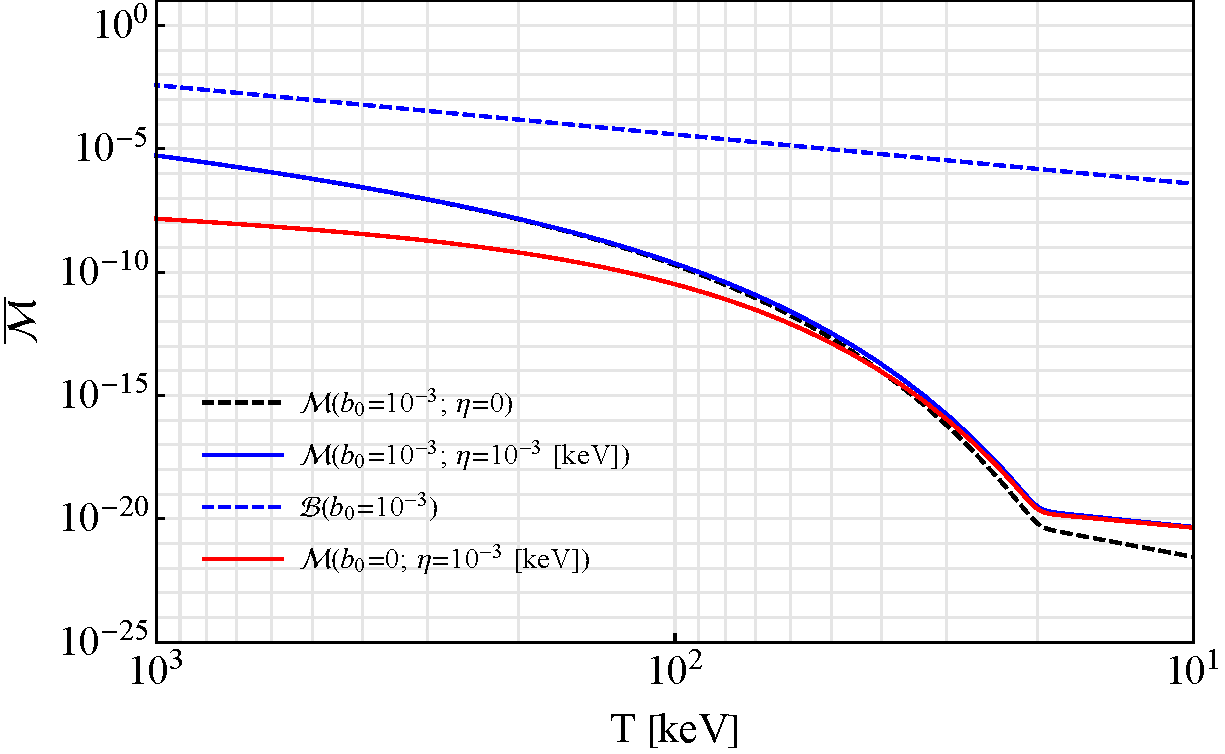
\includegraphics[width=\textwidth]{SpinMidFugacity.pdf}
    \end{subfigure}
    \caption{to be written}
    \label{fig:spin}
\end{figure}
%%%%%%%%%%%%%%%%%%%%%%%%%%%%%%%%%%%%%%%

%%%%%%%%%%%%%%%%%%%%%%%%%%%%%%%%%%%%%%%
\section{Closing}
\label{sec:conclusions}
\noindent to be written
 
MOVE TO CONCLUSIONS\\
This combination of strong magnetic fields, high matter-antimatter density, and relatively high temperatures (far higher than the Sun's core temperature~\cite{bahcall2001solar} of $T_{\odot}=1.37\keV$) make this universe era unique in cosmology and astrophysics.

DELETE OR PLACE ELSEWHERE OR REPHRASE TO KEEP REFERENCE.\\
If the Cosmological Principle is correct~\cite{abdalla2022cosmology}, on the largest scales. Localized inhomogeneities of matter evolution are often non-trivial and generally be solved numerically using magneto-hydrodynamics (MHD)~\cite{melrose2008quantum,vazza2017simulations}.

%%%%%%%%%%%%%%%%%%%%%%%%%%%%%%%%%%%%%%%
\bibliographystyle{unsrtnat}
\bibliography{refs-plasma-partition}
%%%%%%%%%%%%%%%%%%%%%%%%%%%%%%%%%%%%%%%

\end{document}
